\documentclass{article}
\usepackage{hyperref}
\usepackage{float}
\usepackage{verbatim}
\usepackage{placeins}    % for \FloatBarrier
\usepackage{setspace}    % to customize line spacing

% Drawing diagrams
\usepackage{tikz}
\usetikzlibrary{arrows.meta, positioning}

% Language setting
% Replace `english' with e.g. `spanish' to change the document language
\usepackage[english]{babel}

% Set page size and margins
% Replace `letterpaper' with `a4paper' for UK/EU standard size
\usepackage[letterpaper,top=2cm,bottom=2cm,left=3cm,right=3cm,marginparwidth=1.75cm]{geometry}

% Useful packages
\usepackage{amsmath}
\usepackage{graphicx}
\usepackage[colorlinks=true, allcolors=blue]{hyperref}

% Removing Indents & setting line spaces
\setlength{\parindent}{0pt}
\setstretch{1.25}

% Title, Author, Problems/Date
\title{Computer Networks - Homework 3}
\author{JJ McCauley \\ 2/17/25}
\date{Chapter 2's Problems: 3, 14, 27, 28, 36, 40}

\begin{document}
\maketitle

% Question 3
\setcounter{section}{2}
\section{UPD/TCP Checksum Calculation and Error Detection}
We are given three 8-bit bytes: \textbf{01010011}, \textbf{01100110}, and \textbf{01110100}. 

In order to calculate the 1's complement of these three 8-bit bytes, we must first \textit{add them together}. This will give us:
\[
01010011 + 01100110 + 01100110 = 10111001 + 01100110 =  \textbf{1} 00101101
\]
This gives us a 9-but number, but since we are limited to 8 bits, we must wrap around the carry the overflowed number.
\[
00101101 + 00000001 = 00101110
\]
This gives us the sum of the three 8-bit bytes. However, we are asked to find the 1's complement, so we can simply swap the binaries such that:
\[
\text{1's Complement = \textbf{11010001}}
\]
However, the arises the question- Why even take the 1's complement in the first place? Ultimately, UCP/TCP uses 1's complement of the sum because it makes \textbf{error detection easier}. \\

Using the 1's complement allows the receiver to check for errors by \textbf{adding all the received data, including the checksum}. If no errors occurred, the result of the sum should be all 1s, which helps with detecting whether a bit was flipped and detecting other errors that could cancel out with 0s. \textbf{If the result is not all 1s, an error is detected}. \\

Therefore, \textbf{1 bit errors will never go undetected}. \textbf{2-bit errors}, however, \textbf{can sometimes go undetected} as two bits could flip in a way that cancels each other out and make the sum still appear valid.

% Question 14
\setcounter{section}{13}
\section{NAK-Only vs ACK-Based Protocol Efficiency}
We are asked to evaluate NAK-only and ACK-Based protocols for two scenarios: a sender that sends data only infrequently, and a sender that has a lot of data to send and the end-to-end connection experiences few losses.
\subsection{Sending Data Infrequently}
In this scenario, a \textbf{NAK-only protocol} would be preferable. This is because, in this scenario, the sender only sends rarely with data only being sent occasionally, not continuously. Since data is sent infrequently, a NAK-only protocol would send messages only when there is an error, reducing overhead with fewer general control messages and less bandwidth wasted. 
\subsection{Sending Data Frequently with Few Losses}
In this scenario, a \textbf{ACK-based protocol} would be preferable. This scenario presents the sending sending lots of data (high throughput) and few losses (reliable channel). The ACK-based protocol provides feedback with every packet, which would allow for the sender to detect issues sooner if an ACK is missing (especially important with continuous data) and would allow the sender to implement flow and congestion control more effectively. This offers better control and synchronization, improving error recovery and performance.

% Question 27
\setcounter{section}{26}
\section{TCP Segment Ordering \& Acknowledgment Behavior}
We are given a scenario where host A and B are communicating over a TCP connection, with Host B receiving from A all bytes up to byte 126. Host A then sends Host B two segments back-to-back, with the first segment containing 80 bytes and the second containing 40 bytes. In the first segment, the sequence number is 127, the source port number is 302, and the destination port number is 80. Host B sends an acknowledgment whenever it receives a segment from Host A.
\subsection{Sequence \& Port Numbers of the Second Segment}
In order to retrieve the \textit{sequence number}, we must determine the next byte expected (which will be the sequence number). Since we are given the size of the first segment (40 bytes) and the sequence number (127), we can simply add them together such that:
\[
127 + 80 = \textbf{207}
\]
Which will be the sequence number of the second segment. \\

Since we are using TCP, we know that the ports will not change, since everything is transferred within the same connection. Therefore, for the second segment, the \textbf{source port is 302} and the \textbf{destination port is 80}, the same as the first segment.
\subsection{ACK When First Segment Arrives Before Second}
Since TCP acknowledgments are cumulative, the ACK number is the next expected byte. Through the calculations previously executed, we therefore know that the \textbf{ arc number is 207}. \\

Unlike the previous section, ACKs flip the source and destination ports because the reply is going back from Host B to Host A. Therefore, the \textbf{Source Port is 80}, while the \textbf{Destination port is 302}.
\subsection{ACK When Second Segment Arrives Before First}
In this case, Host B has only received up to byte 126 so far. TCP delivers data in order and uses cumulative ACKs, so it will refuse to acknowledge byte 207 (as calculated above) until it receives everything up to byte 206. Therefore, Host B will ignore the out-of-order segment, and \textbf{it will still ACK 127} as it is waiting on the bytes from 127 to 206.
\subsection{TCP Timing Diagram with Lost ACK and Timeout}
\text{\footnotesize Note: LaTeX code generated with ChatGPT 4o.}\\

% Thank you chatGPT for this
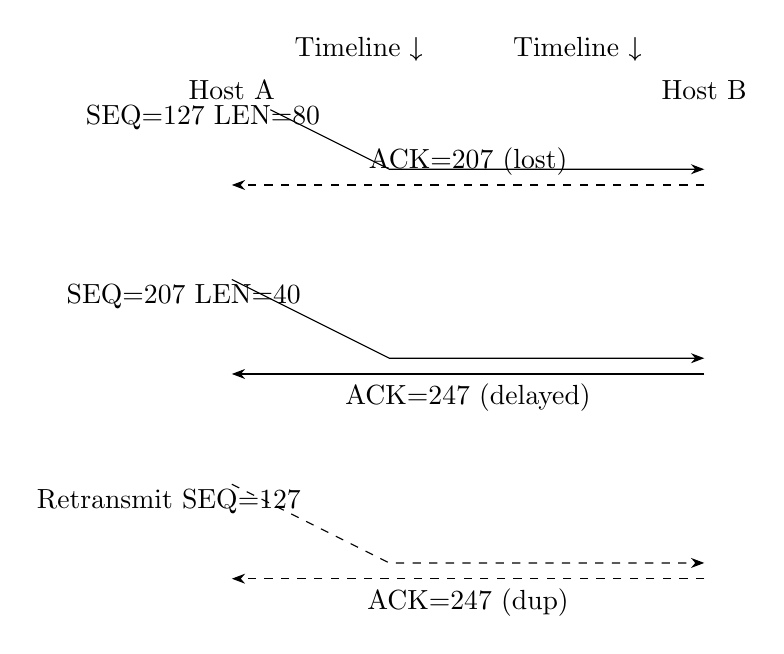
\begin{tikzpicture}[>=Stealth, node distance=1.8cm and 2.5cm]

% Nodes for Host A and B
\node (A) at (0,0) {Host A};
\node (B) at (6,0) {Host B};

% Arrows: SEQ=127, LEN=80
\draw[->] (A) -- ++(2,-1) node[midway, above left] {SEQ=127 \\ \space LEN=80} -- ++(4,0);

% ACK=207 (lost)
\draw[dashed,->] (B) ++(0,-1.2) -- ++(-6,0) node[midway, above] {ACK=207 (lost)};

% Arrows: SEQ=207, LEN=40
\draw[->] (A) ++(0,-2.4) -- ++(2,-1) node[midway, above left] {SEQ=207 \\ \space LEN=40} -- ++(4,0);

% ACK=247 (arrives late)
\draw[->] (B) ++(0,-3.6) -- ++(-6,0) node[midway, below] {ACK=247 (delayed)};

% Timeout and retransmission of SEQ=127
\draw[->, dashed] (A) ++(0,-5) -- ++(2,-1) node[midway, above left] {Retransmit \\ \space SEQ=127} -- ++(4,0);

% Optional duplicate ACK (if B responds again)
\draw[->, dashed] (B) ++(0,-6.2) -- ++(-6,0) node[midway, below] {ACK=247 (dup)};

% Labels for vertical flow
\node[align=center, above right] at (A.north east) {Timeline ↓};
\node[align=center, above left] at (B.north west) {Timeline ↓};

\end{tikzpicture}

% Question 28
\section{TCP Flow Control with Mismatched Send \& Receive Rates}
In this scenario, we are given a link speed (100 Mbps), Host A send rate (Max 120 Mbps), and Host B receive rate (Max 50 Mbps). Clearly, we can see that \textbf{Host B's receive rate} will \textbf{bottleneck the entire TCP connection}. \\
This is due to TCP's \textbf{flow control}, which ensures that the receiving host isn't overwhelmed. TCP uses a receiving window to tell the sender how much buffer space is available from the receiver. When the sender (Host A with a faster sending and link rate) starts sending data into Host B's receive buffer, it will dynamically adjust the receiving window until it becomes 0 when Host B's buffer becomes full. This causes Host A to pause transmission until the contents of the buffer are processed, decreasing any packet loss from Host A overwhelming Host B with data.

% Question 36
\setcounter{section}{35}
\section{Why TCP Waits for Three Duplicate ACKs}




\end{document}